\let\negmedspace\undefined
\let\negthickspace\undefined
\documentclass[journal]{IEEEtran}
\usepackage[a4paper, margin=10mm, onecolumn]{geometry}
\usepackage{lmodern} % Ensure lmodern is loaded for pdflatex
\usepackage{tfrupee} % Include tfrupee package

\setlength{\headheight}{1cm} % Set the height of the header box
\setlength{\headsep}{0mm}  % Set the distance between the header box and the top of the text

\usepackage{gvv-book}
\usepackage{gvv}
\usepackage{cite}
\usepackage{amsmath,amssymb,amsfonts,amsthm}
\usepackage{algorithmic}
\usepackage{graphicx}
\usepackage{float}
\usepackage{textcomp}
\usepackage{xcolor}
\usepackage{txfonts}
\usepackage{listings}
\usepackage{enumitem}
\usepackage{mathtools}
\usepackage{gensymb}
\usepackage{comment}
\usepackage[breaklinks=true]{hyperref}
\usepackage{tkz-euclide} 
\usepackage{listings}
% \usepackage{gvv}                                        
\def\inputGnumericTable{}                                 
\usepackage[latin1]{inputenc}                                
\usepackage{color}                                            
\usepackage{array}                                            
\usepackage{longtable}                                       
\usepackage{calc}                                             
\usepackage{multirow}                                         
\usepackage{hhline}                                           
\usepackage{ifthen}                                           
\usepackage{lscape}
\usepackage{tikz}
\usetikzlibrary{patterns}

\begin{document}

\bibliographystyle{IEEEtran}
\vspace{3cm}

\title{5.2.66}
\author{EE25BTECH11064 - Yojit Manral}

\maketitle
% \maketitle
% \newpage
% \bigskip
{\let\newpage\relax\maketitle}
\renewcommand{\thefigure}{\theenumi}
\renewcommand{\thetable}{\theenumi}
\setlength{\intextsep}{10pt} % Space between text and float

\textbf{Question:}\\
Solve the system of equations
\begin{align}
    2x + 3y = 11 \\
    2x + 4y = -24
\end{align}
Hence, find the value of $m$ for which
\begin{align}
    y = mx + 3
\end{align}

\textbf{Solution:}\\
$\rightarrow$ We have
\begin{align*} \vec{n_1}^T\vec{x} = c_1 && \vec{n_2}^T\vec{x} = c_2 \end{align*}
\begin{align} \implies \myvec{\vec{n_1}^T\\\vec{n_2}^T}\vec{x} = \myvec{c_1\\c_2} \end{align}
$\rightarrow$ From (1) and (2)
\begin{align}
    \vec{n_1} = \myvec{2\\3} && c_1 = 11 \\
    \vec{n_2} = \myvec{2\\4} && c_2 = -24
\end{align}
$\rightarrow$ From (4), (5) and (6)
\begin{align}
    \myvec{2&&3\\2&&4}\vec{x} = \myvec{11\\-24}
    &\xrightarrow{R_2 \leftrightarrow R_2 - R_1} \myvec{2&&3\\0&&1}\vec{x} = \myvec{11\\-35} \\
    &\xrightarrow{R_1 \leftrightarrow R_1 - 3R_2} \myvec{2&&0\\0&&1}\vec{x} = \myvec{116\\-35} \\
    &\xrightarrow{R_1 \leftrightarrow (1/2)R_1} \myvec{1&&0\\0&&1}\vec{x} = \myvec{58\\-35} \\
    &\implies \myvec{x\\y} = \myvec{58\\-35} \implies x = 58 \text{ and } y = -35
\end{align}
$\rightarrow$ From (3)
\begin{align}
    m = \frac{y - 3}{x} = -\frac{19}{29}
\end{align}
\begin{figure}[h!]
   \centering
   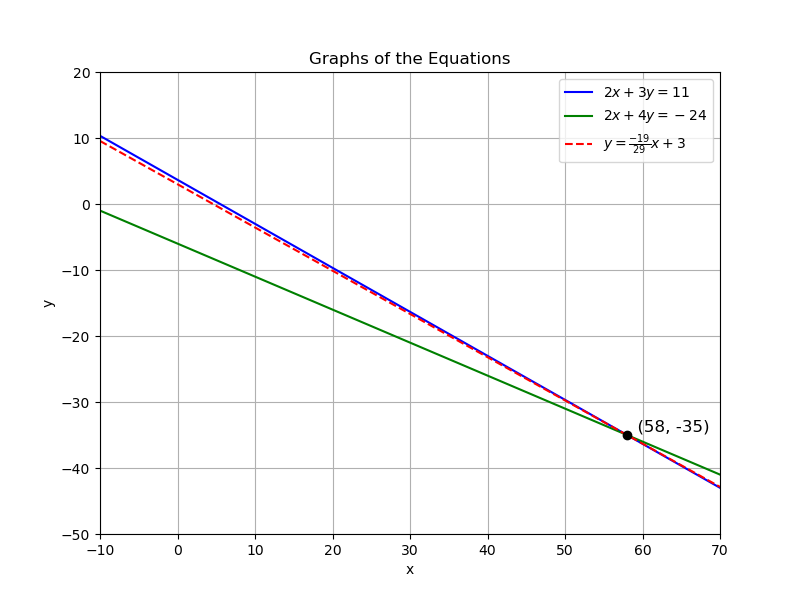
\includegraphics[width=\linewidth]{figs/01.png}
   \caption{Plot of the Equations}
   \label{Plot_1}
\end{figure}
\end{document}
